\documentclass[12pt, a4paper]{article}

\usepackage[polish]{babel}
\usepackage[utf8]{inputenc}
\usepackage{polski}	
\frenchspacing	
\usepackage{graphics}
\usepackage{graphicx}
\usepackage{amsfonts}
\usepackage{amsmath}
\setcounter{secnumdepth}{5}
\usepackage{dirtytalk}
	
	
\title{\textbf{Obliczenia naukowe\\Lista 5}}
\author{Mateusz Kościelniak 244973\\}
\date{Styczeń 2020}

\begin{document}

\maketitle

\newpage

\section{Opis problemu}
Rozwiązanie układu równań liniowych:
\begin{equation}
Ax = b,
\end{equation}
dla danej macierzy $A \in \mathbb{R}^{nxn}$ 
i wektora prawych stron $b \in \mathbb{R}^n$, gdzie $n \geq 4$. \\

\noindent Macierz $A$ jest rzadką macierzą blokową o następującej strukturze:
\begin{equation}
A =
\left(\begin{array}{ccccccc}
A_1 & C_1 & Z & Z & Z & \cdots & Z \\
B_2 & A_2 & C_2 & Z & Z  & \cdots & Z \\
Z  & B_3 & A_3 & C_3 & Z  & \cdots & Z \\
\vdots & \ddots & \ddots & \ddots & \ddots & \ddots & \vdots\\
Z   & \cdots & Z  & B_{v-2} & A_{v-2} & C_{v-2} & Z \\
Z  & \cdots & Z  &  Z &B_{v-1} & A_{v-1} & C_{v-1}  \\
Z  & \cdots & Z & Z & Z& B_{v} & A_{v}  \\
\end{array}\right),
\end{equation} 

\noindent $v = \frac{n}{\ell}$, zakładając że $n$ jest podzielne przez $\ell$, gdzie $\ell \geq 2$ jest rozmiarem wszystkich kwadratowych macierzy wewnętrznych (bloków) $A_i$, $B_i$, $C_i$, $Z$. \\

\noindent Macierze te są następującej postaci:\\

\begin{itemize}
  \item $A_i \in \mathbb{R}^{\ell\times \ell}$,   $i = 1, \ldots,v$ -- macierz gęsta,
  
  \item $B_i \in \mathbb{R}^{\ell\times \ell}$,   $i = 2, \ldots,v$ -- macierz w której dwie ostatnie kolumny są niezerowe:
\begin{equation}
B_i =
\left(\begin{array}{ccccc}
0 & \cdots & 0 & b_{1\,\ell-1}^i & b_{1\,\ell}^i \\
0 & \cdots & 0 & b_{2\,\ell-1}^i & b_{2\,\ell}^i \\
\vdots & & \vdots & \vdots & \vdots \\
0 & \cdots & 0 & b_{\ell\,\ell-1}^i & b_{\ell\,\ell}^i \\
\end{array}\right),
\end{equation} 

\item $C_i \in \mathbb{R}^{\ell\times \ell}$,   $i = 1, \ldots,v\!-\!1$ -- macierz diagonalna:
\begin{equation}
C_i =
\left(\begin{array}{ccccc}
 c_{1}^i & 0 & 0 & \cdots & 0  \\
0 &  c_{2}^i &  0 & \cdots & 0  \\
\vdots &  \ddots &  \ddots & \ddots & \vdots  \\
0 & \cdots & 0 &  c_{\ell-1}^i & 0 \\
0 & \cdots & 0 &  0 & c_{\ell}^i \\
\end{array}\right),
\end{equation} 

\item $Z \in \mathbb{R}^{\ell\times \ell}$ -- macierz zerowa. 
\end{itemize}

\noindent W celu rozwiązania układu równań liniowych $Ax = b$ (1) należało zastosować dwie metody:
\begin{itemize}
\item metodę eliminacji Gaussa w dwóch wersjach, pierwszej bez wyboru elementu głównego oraz drugiej z częściowym wyborem elementu głównego,   
\item obliczyć rozkład~$LU$ macierzy $A$ w wersji bez wyboru elementu głównego oraz z częściowym wyborem elementu głównego, a następnie rozwiązać układ $LUx = b$.
\end{itemize}

\section{Sposób przechowywania macierzy}
Macierz $A$ posiada tylko $(\ell + 3)n - 3 \ell$ elementów nie będących zerami:
\begin{itemize}
\item $v \cdot \ell^2$~w~blokach $A_i$,
\item $(v-1) \cdot 2\ell$ w blokach $B_i$,
\item $(v-1) \cdot\ell$ w blokach~$C_i$.
\end{itemize}
Przechowywanie macierzy A w standardowy sposób (np. zwykła tablica dwuwymiarowa) było by dość nieefektywne ponieważ jest to macierz rzadka. Aby temu zapobiec użyta została specjalna struktura do przechowywania macierzy rzadkich SparseMatrixCSC z języka Julia, w której przechowywane są tylko niezerowe wartości macierzy, wraz z rzędem i kolumną w której leżą.

\section{Opis algorytmów}
\subsection{Metoda eliminacji Gaussa}
\subsubsection{Opis}

W metodzie  eliminacji Gaussa dążymy do stopniowej eliminacji niewiadomych tak aby zastąpić układ równań $Ax=b$ równoważnym mu układem z macierzą trójkątną górną. Końcowy układ równań daje się rozwiązać wprost \say{od dołu}.\\

\noindent Pierwszym krokiem algorytmu eliminacji jest wyzerowanie współczynnika stojącego przy $x_1$ w $n-1$ równaniach leżacych poniżej równania pierwszego poprzez odejmowanie odpowiedniej krotności pierwszego równania od i-tego równania. Przekształcenie to jest zilustrowane poniżej.

\begin{equation}
\left(\begin{array}{cccc|c}
a_{11} & a_{21} & \cdots & a_{n1} & b_1\\
a_{12} & a_{22} &\cdots & a_{n2} & b_2\\
\vdots &  \vdots& & \vdots  & \\
a_{1n} & a_{2n} &\cdots & a_{nn} & b_n\\
\end{array}\right)
\rightarrow
\left(\begin{array}{cccc|c}
a_{11} & a_{21} & \cdots & a_{n1} & b_1\\
0 & y_{22} &\cdots & y_{n2} & z_2\\
\vdots &  \vdots& & \vdots  & \\
0 & y_{2n} &\cdots & y_{nn} & z_n\\
\end{array}\right)
\end{equation} \\

\noindent Takie postępowanie powtarzane jest dla kolejnych niewiadomych $x_{j}$, gdzie od $i$-tego równania odejmowana jest odpowiednia krotność $j$-tego równania dla $i = j+1, \cdots, n$. Na końcu dostajemy następującą macierz:\\

\begin{equation}
\left(\begin{array}{ccccc|c}
a_{11} & a_{21} & y_{31} & \cdots & a_{n1} & b_1\\
0      & y_{22} & y_{23} & \cdots & y_{n2} & z_2\\
0      & 0      & y_{33} & \cdots & y_{n3} & z_3\\
\vdots & \vdots &        &        & \vdots & \\
0      & 0      & 0      & \cdots & y_{nn} & z_n\\
\end{array}\right)
\end{equation} \\

\noindent Widzimy, że pod diagonalą występują tylko elementy o wartościach równych zeru. W ostanim kroku rozwiązujemy powstały układ z macierzą trójkątną górną algorytmem podstawiania wstecz, polegającym na obliczeniu:

$$
x_i = \frac{b_i - \sum_{j = i+1}^n a_{ij}}{a_{ii}}
$$
\begin{itemize}
\item[$x_i$]-- i-ta niewiadoma
\item[$b_i$]-- wartość i-tej skladowej wektora prawych stron
\item[$a_{ij}$]-- składowa macierzy A
\item[]dla wierszy $i$ od $n$ do $1$.
\end{itemize}

\noindent Aby wykonać tą procedure trzeba przyjąć założenie, że każdy element macierzy leżący na jej diagonali jest różny od zera. W przypadku kiedy macierz niespełnia takiego założenia konieczna jest modyfikacja algorytmu. Jeśli $i$-tym kroku napotkamy element równy zeru wyszukujemy w $i$-tej kolumnie element (zwany elementem głównym) o największej co do modułu wartości po czym wiersz z tym elementem zamieniamy miejscem z $i$-tym wierszem. Taka zamiana zawsze jest możliwa, gdyż w przeciwnym przypadku macierz byłaby osobliwa. \\

\subsubsection*{Złożoność}
Złożoność opisanej powyżej metody  eliminacji Gaussa wynosi
$O(n^3)$, natomiast algorytmu podstawiania wstecz $O(n^2)$, zatem całkowita złożoność algorytmu rozwiązującego układ równan to $O(n^3)$

\subsubsection{Optymalizacje}

Macierz którą zajmujemy się w tym zadaniu jest macierzą rzadką, ponadto ma specyficzną blokową postać, co w pewnym stopniu umożliwia zredukowanie wykonywanych operacji. Można również zauwarzyć, że wiele elementów macierzy $A$ leżących pod diagonalą jest już zerami i nie ma potrzeby ponownego ich zerowania. Widzimy, że w macierzy $A$ ostatnim niezerowym elementem w każdym wierszu poza ostatnimi blokiem jest element leżący na diagonali bloku $C_i$, ponadto element ten znajduje się zawsze w odległości $\ell$ od elementu na diagonali macierzy $A$. Ta obserwacja pozwala wyprowadzić wzór na indeks kolumny z ostatnim niezerowym elementem w wierszu, wygląda on następująco: 

\begin{equation}
k_{max}(r) = \min\{r + \ell, n\}.
\end{equation}
\begin{itemize}
\item[$k_{max}$]-- kolumna z ostatnim niezerowym elementem
\item[$r$] -- wiersz
\end{itemize}

\noindent Można również zauwarzyć, że dla pierwszych $\ell-2$ kolumn elementy niezerowe będą się znajdowały jedynie w bloku $A_1$, czyli w $\ell$ pierwszych rzędach, natomiast dla  kolejnych kolumn w bloku, elementy niezerowe będą najniżej w bloku $B_2$. Schemat ten powtarza się w kolejnych blokach co za tym idzie można wyprowadzć wzór na indeks ostatniego niezerowego elementu w danej kolumnie, wygląda on następująco:

\begin{equation}
r_{min}(k) = \min\left(n, \, \ell + \ell \cdot \left \lfloor\frac{k + 1}{\ell}\right \rfloor\right)
\end{equation}
\begin{itemize}
\item[$r_{min}$] -- wiersz z ostatnim niezerowym elementem
\item[$k$] -- kolumna
\end{itemize}

\noindent Algorytm podstawiania wstecz również można poddać drobnym modyfikacjom wykorzystując fakt, że w wyniku eliminacji Gaussa poza elementami pod diagonalą bloków $C_i$ w macierzy $A$ nie powstały żadne nowe elementy niezerowe, dlatego wystarczy dla każdego wiersza sumować elementy tylko do pewnej kolumny określonej wyprowadzonym wcześniej wzorem (7). \\

\subsubsection*{Złożonoś bez wyboru elementu głównego}
Po modyfikacji złożoność metody eliminacji Gaussa, wynosi $O(n)$. Zewnętrzna pętla wykonuje $n-1$ przebiegów, środkowa maksymalnie $2\ell$, natomiast wewnętrzna maksymalnie $\ell$. Z kolei w algorytmie podstawiania wstecz zewnętrzna pętla wykonuje $n$ przebiegów, natomiast wewnętrzna maksymalnie $\ell$. Jest to znacząca poprawa względem standardowej metody eliminacji Gaussa.\\

\noindent Teraz rozpatrzmy wariant algorytmu z wyborem elementu głównego, tutaj normalny algorytm eliminacji Gaussa posługuje się zamianą wierszy, lecz w praktyce taka zamiana bywa kosztowna, szczególnie kiedy operacje wykonywane są na dużych macierzach, dlatego będziemy się tutaj posługować wektorem permutacji wierszy. W tym wektorze pamiętane jest na jakiej aktualnie pozycji w macierzy znajduje się dany wiersz, więc zamiast odwoływać się do konkretnego wiersza w macierzy A, odwołamy się do jego pozycji w wektorze permutacji. Z wyborem elementu głownego wiąże się rownież problem z zachowaniem dotychczas wyliczonych wartości $c_{max}$ (równanie (7)), ponieważ wiersze odejmowane są w innej kolejności, może to doprowadzić do  powstania nowych elementów niezerowych. Musimy więc oszacować $c_{max}$ w inny sposób. Widzimy, że podczas eliminowania współczynników z $\ell - 2$ pierwszych kolumn najdalszy niezerowy element można stworzyć w kolumnie z indeksem $2\ell$, poprzez odejmowanie $\ell$-tego wiersza, który w tej kolumnie posiada niezerowy element.
Następnie eliminując współczynniki w kolejnych $\ell$ kolumnach najdalszy niezerowy element można stworzyć w kolumnie z indeksem $3\ell$, analogicznie poprzez odejmowanie $2\ell$-tego wiersza, który w tej kolumnie posiada niezerowy element. To rozumowanie pozwala nam uzyskać nowy wzór:


\begin{equation}
k'_{max}(k) = \min\left\lbrace2\ell + \ell \cdot \left \lfloor\frac{k + 1}{\ell}\right \rfloor, n\right\rbrace
\end{equation}



\noindent W algorytmie podstawiania wstecz zastosowane jest podobne ograniczenie, dodatkowo musimy pamiętać o uwzględnieniu permutacji wierza.\\

\subsubsection*{Złożonoś z wyborem elementu głównego}
Ogólnie z powodu zastosowania szerszych ograniczeń $k'_{max}$ złożoność jest tego algorytmu z częściowym wyborem elementu głównego jest nieco gorsza, lecz nie wpływa to na końcową złożoność asymptotyczną która nadal wynosi $O(n)$.

\subsection{Metoda z rozkładem LU}
\subsubsection{Opis}
Ideą rozkładu ${LU}$ macierzy $A$ jest przedstawienie jej za pomocą iloczynu
\begin{equation}
A = LU
\end{equation}
gdzie,
\begin{itemize}
\item[$L$] -- macierz trójkątna dolna,
\item[$U$] -- macierz trójkątna górna.
\end{itemize}

\noindent Rozkład $LU$ możemy uzyskać za pomocą używanej wcześniej metody eliminacji Gaussa która przekształca macierz $A$ do macierzy trójkątnej górnej, więc mamy już macierz U. Aby otrzymać macież $L$ musimy zapamiętać mnożniki użyte do eliminacji kolejnych współczynników macierzy $A$, mianowicie mnożnik użyty do wyzerowania elementu $a_{ij}$ macierzy $A$ będzie zapisany w i-tym wierszu i j-tej kolumnie macierzy $L$. Dodatkowo cały rozkład $LU$ możemy zapisać w macierzy A oszczędzając w ten sposób pamięć. Dalsza część algorytmu rozwiązujemy dwa równania z wyznaczonymi wczęśniej macierzami:

\begin{subequations}
\begin{equation}
Lz = b
\end{equation}
\begin{equation}
Ux = z
\end{equation}
\end{subequations}

\subsubsection*{Złożoność}
Złożoność obliczeniowa wyznaczenia rozkładu $LU$ to $O(n^3)$, natomiast dalsza część polegająca na rozwiązaniu równań 11a i 11b to $O(n^2)$, zatem całkowita złożoność tej metody jest równa $O(n^3)$.

\subsubsection{Optymalizacje}

Początkowe etapy algorytmu, a mianowicie wyznaczanie rozkładu $LU$ są podobne do metody eliminacji Gaussa, z tą różnicą, że zamiast zerowania elementów poniżej diagonali podstawiane są mnożniki, stanowiące element macieży $L$.

\noindent W następnym etapie rozwiązujemy dwa równania Lz = b oraz Ux = z. Dla drugiego równania z kolei, stosujemy algorytm podstawiania wstecz który omawiany był przy opisie metody eliminacji Gaussa, natomiast dla pierwszego równania czyli 
Lz = b, należy zastosować algorytm podstawiania w przód, który jest podobny do algorytmu podstawiania wstecz, z tą różnicą, że zaczynamy od pierwszego wiersza i sumowane są elementy z kolumn coraz dalszych. Ze względu na specyficzną postać macierzy nie musimy sumować od pierwszej kolumny, lecz możemy wyprowadzić wzór na najmniejszy indeks kolumny z elementem niezerowym, który wygląda następująco:

\begin{equation}
k_{min}(r) = \max\left\lbrace\ell \cdot \left \lfloor\frac{r - 1}{\ell}\right \rfloor - 1, 1 \right\rbrace.
\end{equation}

\noindent W przypadk algorytmu z częsciowym wyborem elementu głównego, sytuacja jest identyczna jak w metodzie eliminacji Gaussa z wyborem elementu głównego, również zamiast odwoływania się do konkretnego wiersza, następuje odwołanie do jego pozycji w wektorze permutacji.

\subsubsection*{Złożoność}
Dla etapu wyznaczania rozkładu $LU$, złożoność jest taka sama, jak przy metodzie eliminacji Gaussa i wynosi $O(n)$. Wiemy również, że równanie $Ux = z$ obliczamy w zasadzie taki samym sposobem jak w metodzie eliminacji Gaussa co za tym idzie złożoność będzie wynosiła również $O(n)$ tak samo będzie w przypadku równania Lz = b, ponieważ algorytmy podstawiania w przód oraz wstecz są bardzo podobne, z różnicami nie wpływającymi na złożoność. Całkowita złożoność obliczeniowa dwóch przedstawionych powyżej algorytmów będzie wynosiła $O(n)$.

\section{Wyniki}

We wszystkich przedstawianych wynikach przyjęto rozmiar bloku $\ell = 4$.

\begin{table}[!h]
        \centering
        \footnotesize
\begin{tabular}{c|c|c|c|c}
& \multicolumn{2}{c|}{bez wyboru} & \multicolumn{2}{c}{z wyborem}\\
\hline
n & czas & pamięć & czas & pamięć\\
\hline
16 & 2.196825e-5 s & 1.765625 KiB & 3.572125e-5 s & 1.96875 KiB\\
100 & 0.00011808125 s & 11.625 KiB & 0.00027630275 s & 12.5 KiB\\
1000 & 0.00168473675 s & 117.125 KiB & 0.007516448 s & 125.0625 KiB\\
5000 & 0.020702967 s & 585.828125 KiB & 0.1219524235 s & 624.96875 KiB\\
10000 & 0.072240278 s & 1171.765625 KiB & 0.4197928775 s & 1249.96875 KiB\\
20000 & 0.27308202675 s & 2343.640625 KiB & 1.5781400777499999 s & 2499.96875 KiB\\
50000 & 17.543526932500003 s & 5859.265625 KiB & 21.55172780225 s & 6249.96875 KiB
\end{tabular}
\caption{Tabela średniego czasu wykonywania i średniej zużytej pamięci dla metody eliminacji Gaussa  w wariancie bez wyboru elementu głównego i z jego częściowym wyborem.}
\end{table}

\begin{table}[!h]
        \centering
        \footnotesize
\begin{tabular}{c|c|c|c|c}
& \multicolumn{2}{c|}{bez wyboru} & \multicolumn{2}{c}{z wyborem}\\
\hline
n & czas & pamięć & czas & pamięć\\
\hline
16 & 2.15985e-5 s & 1.96875 KiB & 3.871525e-5 s & 2.18359375 KiB \\
100 & 0.000111983 s & 12.5 KiB & 0.000261098 s & 13.38671875 KiB\\
1000 & 0.001587229 s & 125.0625 KiB & 0.005927278500000001 s & 133.01171875 KiB\\
5000 & 0.02026969375 s & 624.96875 KiB & 0.107517222 s & 664.12109375 KiB\\
10000 & 0.07104080625 s & 1249.96875 KiB & 0.408460537 s & 1328.18359375 KiB\\ 
20000 & 0.261626478 s & 2499.96875 KiB & 1.56150060975 s & 2656.30859375 KiB \\
50000 & 17.3710081715 s & 6249.96875 KiB & 22.403721522249995 s & 6640.68359375 KiB 
\end{tabular}
\caption{Tabela średniego czasu wykonywania i średniej zużytej pamięci dla metody LU  w wariancie bez wyboru elementu głównego i z jego częściowym wyborem.}
\end{table}


\begin{figure}[!h]
\centering
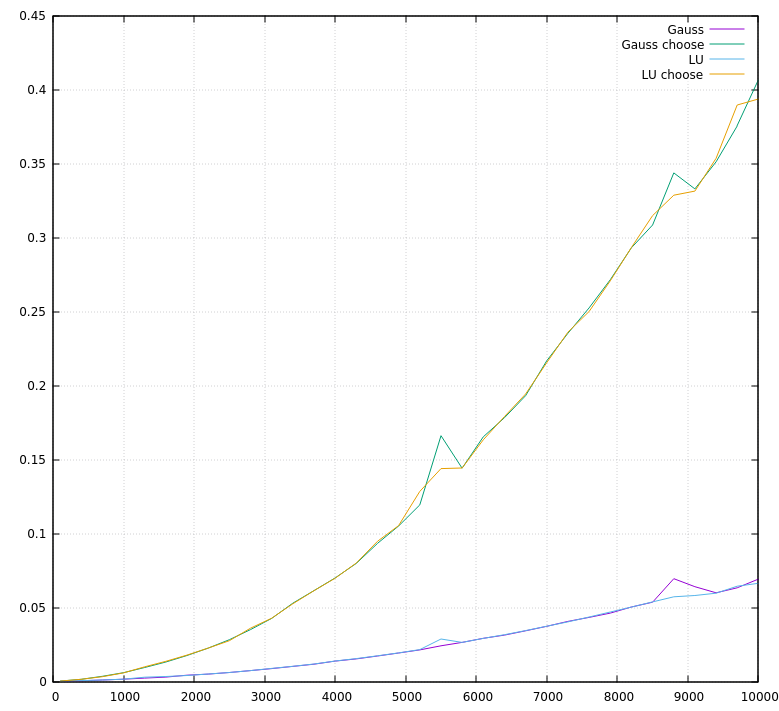
\includegraphics[width=400px]{timePlot.png}
\caption{Wykres czasów wykonywania algorytmów od wielkości macierzy.}
\end{figure} 	


\begin{table}[!h]
        \centering
        \footnotesize
\begin{tabular}{c|c|c|c|c}
n & bez wyboru & z wyborem\\
\hline
16 &  3.107895799689565e-14 & 3.433175098891678e-16 \\
100 &  2.949121011348651e-15 & 2.6107951392584033e-16 \\
1000 &  2.9256114662419202e-15 & 3.0136983042333716e-16 \\
5000 &  1.96505177640419e-14 & 3.000171026473022e-16 \\
20000 &  4.459026580959929e-14 & 2.98232852765259e-16 \\
50000 &  4.503491569922606e-14 & 3.005195520712902e-16 
\end{tabular}
\caption{Zestawienie błędów względnych dla metody eliminacji Gaussa.}
\end{table}
Widzimy, że błędy w metodzie z wyborem elementu głównego są prawie o rząd wielkości mniejsze, taka prawidłowość zachodzi również w metodach z rozkładem LU.

\section{Wnioski}
Przedstawione wyniki pokazują, że rzeczywiście złożoność obliczeniowa zaimplementowanych metod jest liniowa. 
Możemy zobaczyć, że wolniejsza i zużywająca większą ilość pamięci metoda z częściowym wyborem elementu głównego zarówno w metodzie eliminacji Gaussa jak i w rozkładzie $LU$ jest ona jendak bardziej uniwersalna, pozwala nam rozwiązać układ w przypadku elementów zerowych na diagonali. Po wykresie czasów widzimy, żę metoda z rozkładem  LU jest nie co gorsza od metody eliminacji Gaussa, jednak kiedy dla jednej macierzy pojawia się więcej różnych wektorów prawych stron ta metoda staje się bardzo opłacalna, ponieważ sam rozkład macierzy jest liczony tylko raz, a rozwiązanie układu z dwóch macierzy trójkątnych jest szybsze i łatwiejsze niż przeprowadzenie eliminacji Gaussa od początku. Eksperymenty pokazują również, że przeprowadzone optymalizacje pod kątem specyficznej macierzy przyniosły dobry skutek. Dzięki optymalizacjom, zlożoność algorytmów z $O(n^3)$ zmniejszyła się do O(n), co za tym idzie, możemy mnożyć większe macierze w krótszym czasie przy mniejszym zużyciu pamięci, zatem widać jak ważna jest optymalizacja algorytmów pod kątem konkretnych przypadków. 

\end{document}
